\section{Optimizing Pointwise Convolution}
In this section, we first demonstrate how to distribute input channels among threads within a warp. 
Then, we describe how to determine the threads to calculate one input elements.
\subsection{Distribute Input Channels}
Pointwise convolution has a low arithmetic intensity compared with multi-channel 2D convolution. 
Especially when performing training or inference in batch sizes of 64, 32, 16, etc.
However, the pointwise convolution implementation of cuDNN is inefficient in this situation. 
They choose a fixed blocking strategy for convolutions with high and low arithmetic intensity. 
However, blocking strategy which is suitable for high arithmetic intensity will result in GPU underutilization since there is not enough output elements to keep all CUDA cores busy.
To address this problem, we design a dynamic blocking strategy for low arithmetic intensity pointwise convolution that will calculate block size based on output size and hardware limits and yet can hide memory access latency.
The main idea is to let different number of threads to calculate one output elements for different arithmetic intensity.

First, we fix the size of thread block to 4 warps (each warp contains 32 threads). More warps will decrease the block number and may hurt GPU utilization. 
Next, based on the number of SM, we calculate how many output elements each SM needs to process to fully utilize GPU.
The key issue here is to find a value that can increase the arithmetic intensity as well as GPU utilization. 
We give two choices for SM, each SM calculates 2 blocks or 4 blocks, which corresponding to 128 registers per thread or 255 (each thread at most have 255 registers) registers per thread.
We calculate how many output elements each thread block needs to process.
The most difficult part is how to map block tile into warps and threads.
We use two mappings to map thread blocks into output elements.
Now, for each mapping, we can decide how many filters each warp needs to calculate and therefor, how many inputs each warp to calculate.
Now we iterate over all possible channel numbers (1, 2, 4, 8, 16 and 32) to find a filter number that do not exceed half of registers available under this mapping and most close to input number.
Last, we choose the best configurations from all possible ones.
\begin{figure}
	\centering
    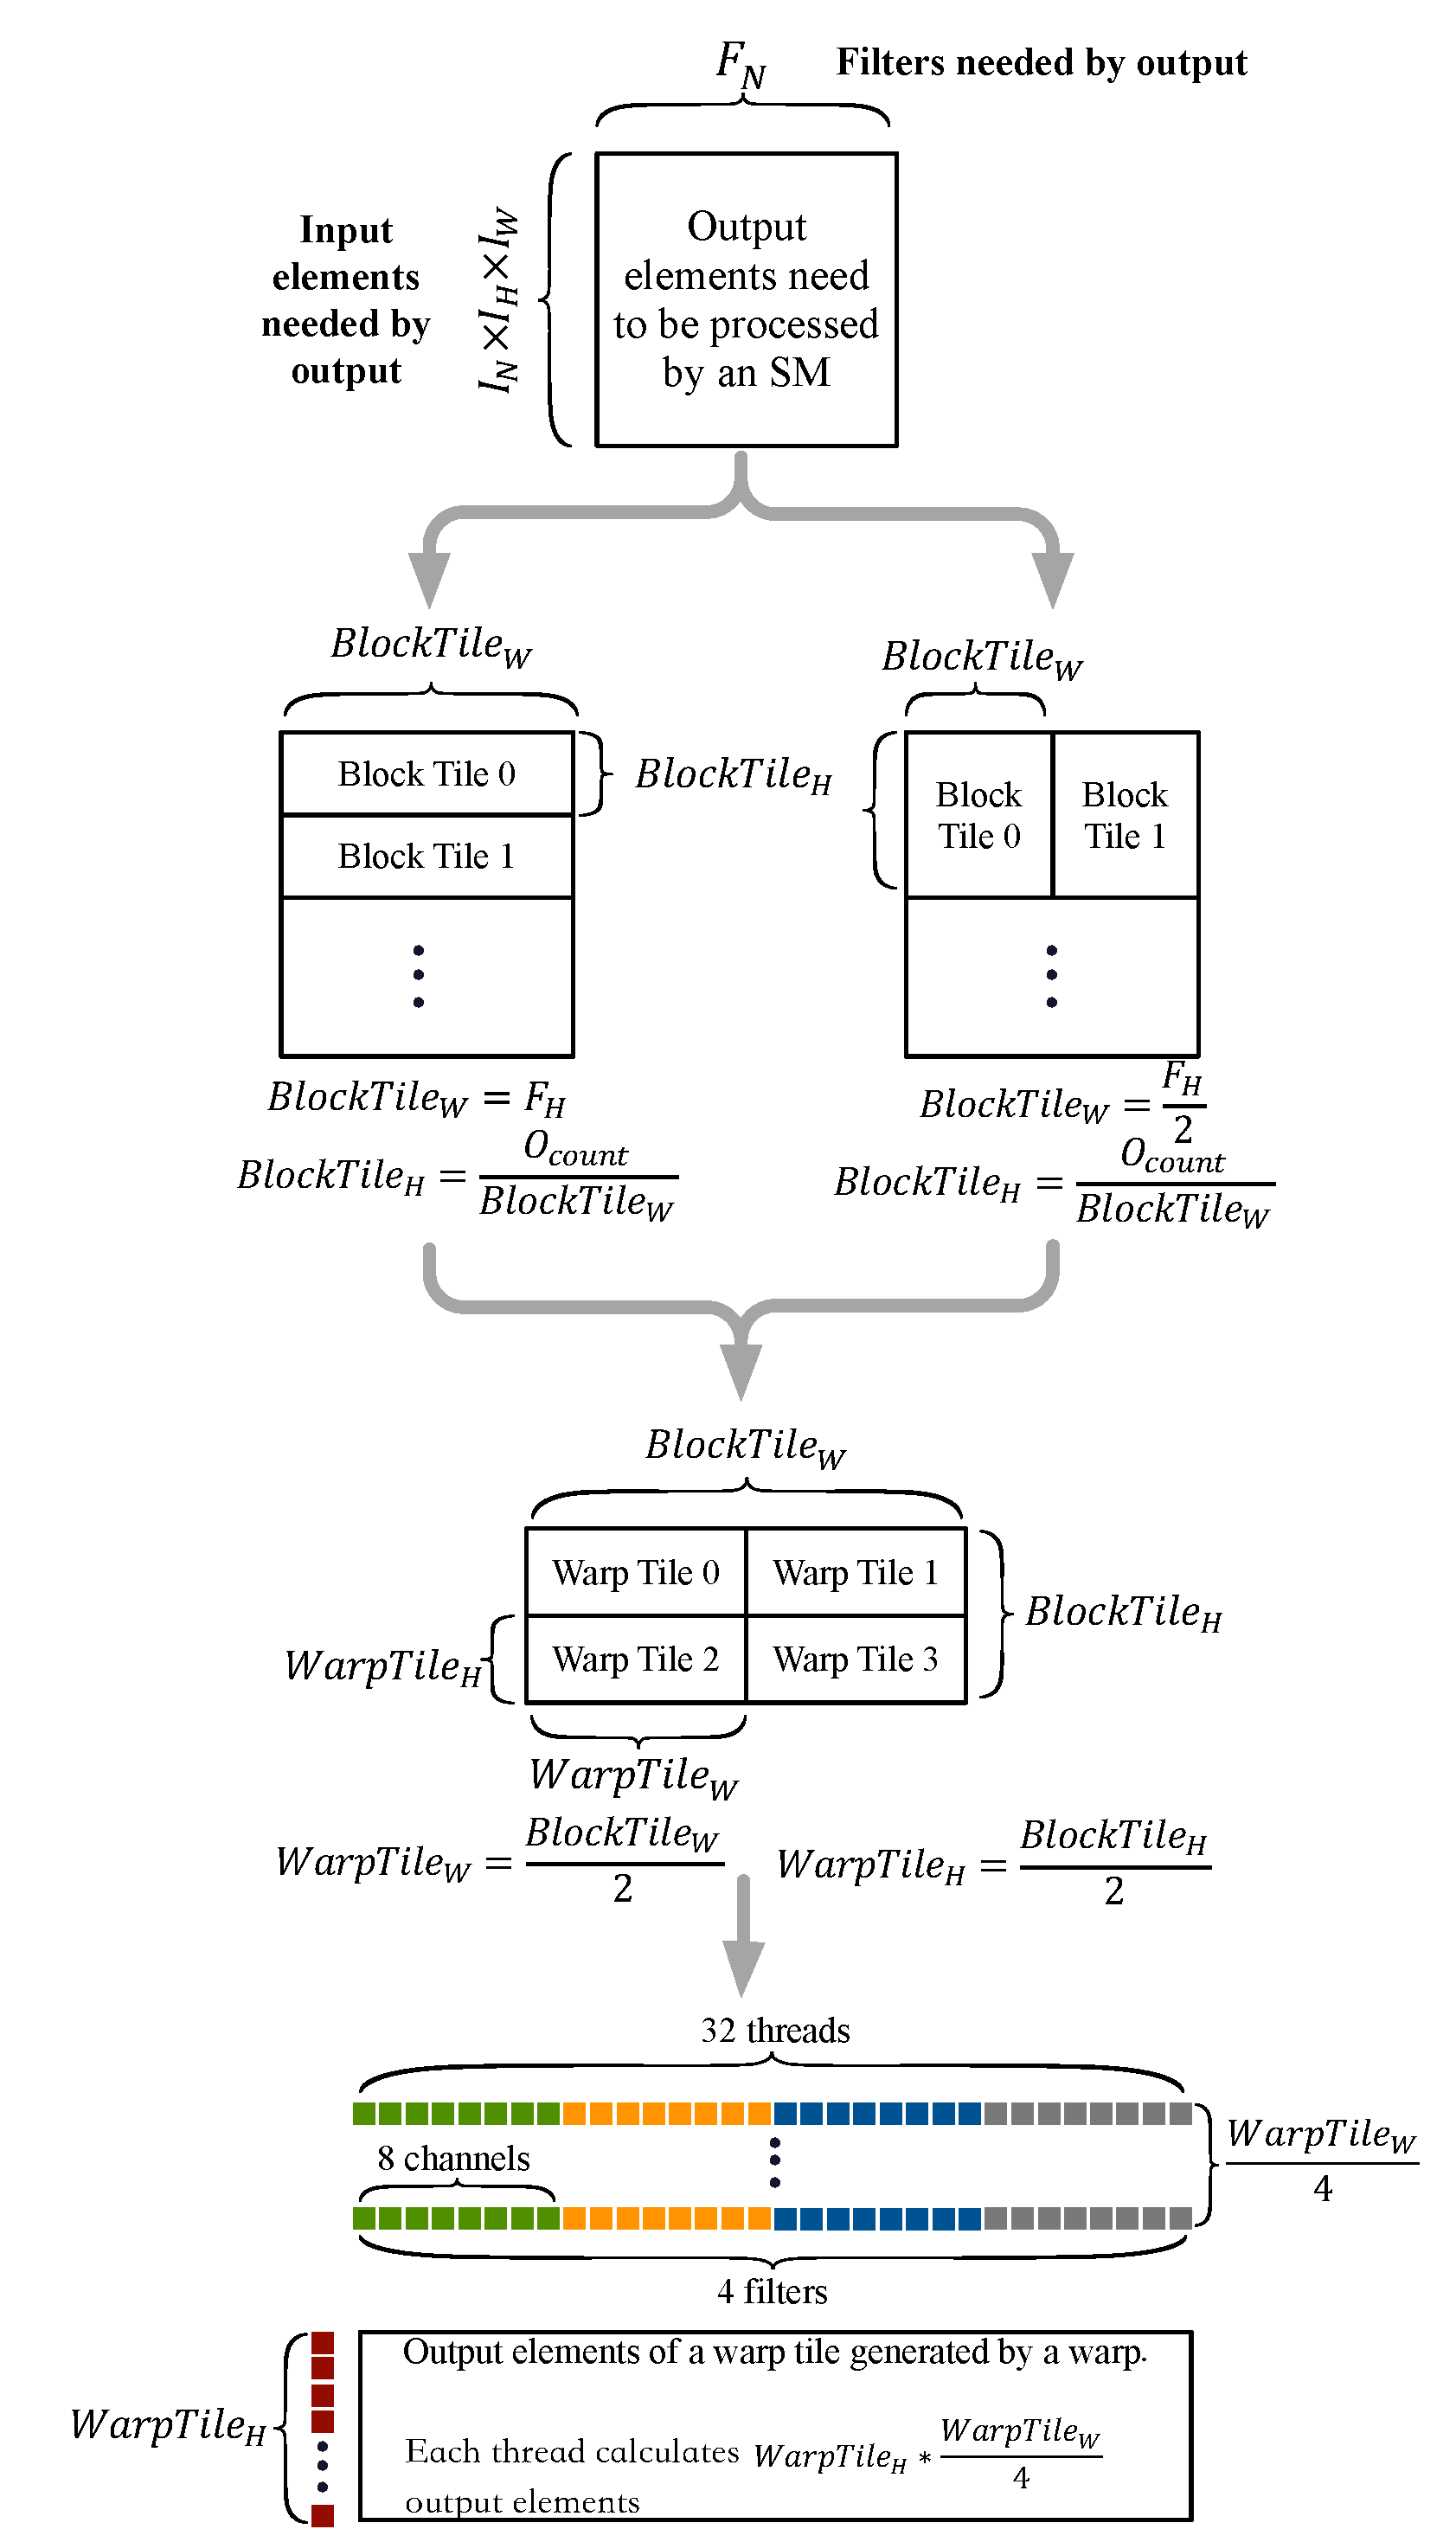
\includegraphics[width=\columnwidth]{./figure/pwflow.eps}
    \caption{} \label{fig:pwflow}
\end{figure}
\begin{algorithm}[t!]
    \small
        \KwIn{$I$, $F$}
        \KwOut{$O$}
        Calculate how many output elements one SM needs to process if we want to fully utilize GPU, denoted as $O_{sm}$\;
        \tcp{below codes are executed on CPU}
        \tcp{we have two options for block tile number, one SM contains 2 or 4 block tiles}
        \ForEach{block tile number of one SM}{
            Use $BlockTile_{count}$ to denote the number of block tiles resided on one SM\;
            \ForEach{block layout}{
                Calculate the width of a block tile, denoted as $BlockTile_W$\;
                $BlockTile_H = \frac{O_{sm}}{BlockTile_W * BlockTile_{count}}$\;
                \If{$BlockTile_H > 32$}{
                    $niter = BlockTile_H/32$\;
                    $BlockTile_H = 32$\;
                }
                $WarpTile_H=\frac{BlockTile_H}{2}$\;
                $WarpTile_W=\frac{BlockTile_W}{2}$\;
                \tcp{there are 6 choices for channel count, 1,2,4,8,16,32}
                \ForEach{channel count}{
                    Use $C_{count}$ to denote how many threads are uesed to calculate channels of the same output element.\;
                    $filter_{num} = \frac{32}{C_{count}}$\;
                    $filter_{num} = \frac{WarpTile_W}{filter_{num}}$\;
                    Calculate registers and shared memory usage under this configuration, and evaluate if the usage not exceeds the limit.\;
                    record the configuration with smallest register usage. 
                }
            }
        }
        \tcp{below codes are executed on GPU}
        All threads in a thread block cooperate to load the needed input and filter into shared memory\;
        $\_\_syncthreads()$\;
        \For{$iter \gets 0$ \KwTo $I_C$ By $C_{count}$}{
            load next $C_{count}$ channels for input and filter into registers\;
            load current channels of input and filter into registers\;
            calculate output elements\;
            write registers of next channels into shared memory\;
        }
        use segmented parallel reduce to get the final output elements and write the result to global memory\;
        \caption{Pointwise Convolution Optimization}
        \label{algo:pwalgo}
\end{algorithm}